\documentclass[12pt]{article}
\usepackage{fullpage,graphicx,psfrag,color}

\input defs.tex

\bibliographystyle{alpha}

\title{Computing the Arrow-Debreu Market Equilibrium}
\author{}

\begin{document}

\maketitle

\section{Introduction}

We have a market with $m$ agents and $n$ goods. Agent $i$
initially has amount $b_{ij}$ of good $j$. Agent $i$ achieves
utility $a_{ij} x_{ij}$ when he is allocated amount $x_{ij}$
of good $j$. Thus agent $i$'s total utility is $\sum_j a_{ij}x_{ij}$
when he is allocated $(x_{i1},\ldots,x_{in})$.

A market equilibrium is a set of allocations of goods
to agents $x_{ij}$ together with a set of good prices $p \in \reals^n$
such that at equilibrium
\BIT
\item all goods are sold at the equilibrium price.
\item each agent maximizes his total utility. 
\EIT
It can be shown that a market equilibrium always exists and can be
found by solving the following problem
\BEQ\label{e-eq_prob}
\begin{array}{ll}
\mbox{find} & x, \quad p\\
\mbox{subject to} & \sum_k a_{ik} x_{ik} \geq a_{ij} \sum_{k} b_{ik} \frac{p_k}{p_j}, 
                    \quad \forall \; i,j\\
                  & \sum_i x_{ij} = \sum_i b_{ij}, \quad \forall j\\
                  & x_{ij} \geq 0, \quad p_j \geq 0. 
\end{array}
\EEQ

Problem (\ref{e-eq_prob}) is not a convex optimization problem but can
be easily transformed to one by a simple change of variables.
Specifically let $p_j = \exp(\psi_j)$. Then problem (\ref{e-eq_prob})
becomes
\BEQ\label{e-eq_prob_cvx}
\begin{array}{ll}
\mbox{find} & x, \quad \psi\\
\mbox{subject to} & \sum_k a_{ik} x_{ik} \geq a_{ij} \sum_{k} b_{ik} e^{\psi_k-\psi_j}, 
                    \quad \forall \; i,j\\
                  & \sum_i x_{ij} = \sum_i b_{ij}, \quad \forall j\\
                  & x_{ij} \geq 0.
\end{array}
\EEQ
This is a convex feasibility problem and can be solved in a
variety of ways. In fact this is a mixed linear-GP.

\section{A Trust Region Solution}

In this section we describe a simple trust region style method for
solving problem (\ref{e-eq_prob_cvx}). This method proceeds in the following
way: given an infeasible point $(x,\psi)$, we linearize the first set of
constraints in (\ref{e-eq_prob_cvx}) about this point. We allow our
next operating point to deviate by a small amount about the previous
operating point (the so-called trust region) and update our point
accordingly

We first start by reformulating
(\ref{e-eq_prob_cvx}) as the following optimization problem
\BEQ\label{e-eq_prob_cvx2}
\begin{array}{ll}
\mbox{maximize} & \min t_i\\
\mbox{subject to} & t_i \leq \sum_k a_{ik} x_{ik} - a_{ij} \sum_{k} b_{ik} e^{\psi_k-\psi_j}, 
                    \quad \forall \; i,j\\
                  & \sum_i x_{ij} = \sum_i b_{ij}, \quad \forall j\\
                  & x_{ij} \geq 0, 
\end{array}
\EEQ
where the optimization variables are $x$, $t$, and $\psi$. Note that this
problem is equivalent to (\ref{e-eq_prob_cvx}) since a
market equilibrium always exists.

Now, given $\psi$, we linearize the first set of constraints of 
(\ref{e-eq_prob_cvx2}), which gives the following problem
\BEQ\label{e-delta_psi}
\begin{array}{ll}
\mbox{maximize} & \min t_i\\
\mbox{subject to} & t_i \leq \sum_k a_{ik} x_{ik} - a_{ij} \left(\sum_{k} b_{ik} 
                    e^{\psi_k-\psi_j}(1+\Delta \psi_k - \Delta \psi_j)
                    -b_{ij} \Delta \psi_j\right), 
                    \quad \forall \; i,j\\
                  & \sum_i x_{ij} = \sum_i b_{ij}, \quad \forall j\\
		  & \sum_j \Delta \psi_j = 0, \quad \|\Delta \psi\|_\infty \leq \Delta_\mathrm{max} \\ 
                  & x_{ij} \geq 0, 
\end{array}
\EEQ
with variables $x$, $t$, and $\Delta \psi$. We put a constraint
in the sum of $\Delta \psi_j$ since the $\psi_j$'s are invariant
to scalar shifting. The parameter $\Delta_\mathrm{max}$ controls
the width of the trust region. 

This is an LP and can be
solved using an off-the-shelf solver. 
In fact if $a$ and $b$ are sparse, then we can easily write
a custom LP solver that can deal with large instances of this problem.

Given a current operating point $(x,\psi)$ we define the
{\em agent residual} $\eta$ as
\[
\eta = \min_{i,j}\left(\sum_k a_{ik} x_{ik} -
 a_{ij} \sum_{k} b_{ik} e^{\psi_k-\psi_j}\right).
\]

The trust region algorithm for solving problem (\ref{e-eq_prob_cvx})
proceeds as follows
\begin{algdesc}
\begin{tabbing}
{\bf given} tolerance $\epsilon >0$, parameter $\Delta_\mathrm{max}$,
\\*[\smallskipamount]
{initialize:} $\psi = 0$
\\*[\smallskipamount]
{\bf while}  $\eta < -\epsilon$\\*[\smallskipamount]
\qquad \= compute $(x,\Delta \psi)$ from (\ref{e-delta_psi})\\
\>update:\\
\> \qquad \= $\psi:= \psi + \Delta \psi$
\end{tabbing}
\end{algdesc}

We generated a simple numerical example with $m = 30$
$n = 30$ and with $a_{ij}$, $b_{ij}$ random,
uniformly distributed between $0$ and $1$.
We set $\Delta_\mathrm{max} = 0.1$ and $\epsilon = 10^{-8}$. 

Figure \ref{f-agent_res} shows the agent residual versus
algorithm iteration for an instance of this problem.

\begin{figure}
\begin{center}
\psfrag{agentres}[b][t]{Agent residual}
\psfrag{iter}[t][b]{Iteration}
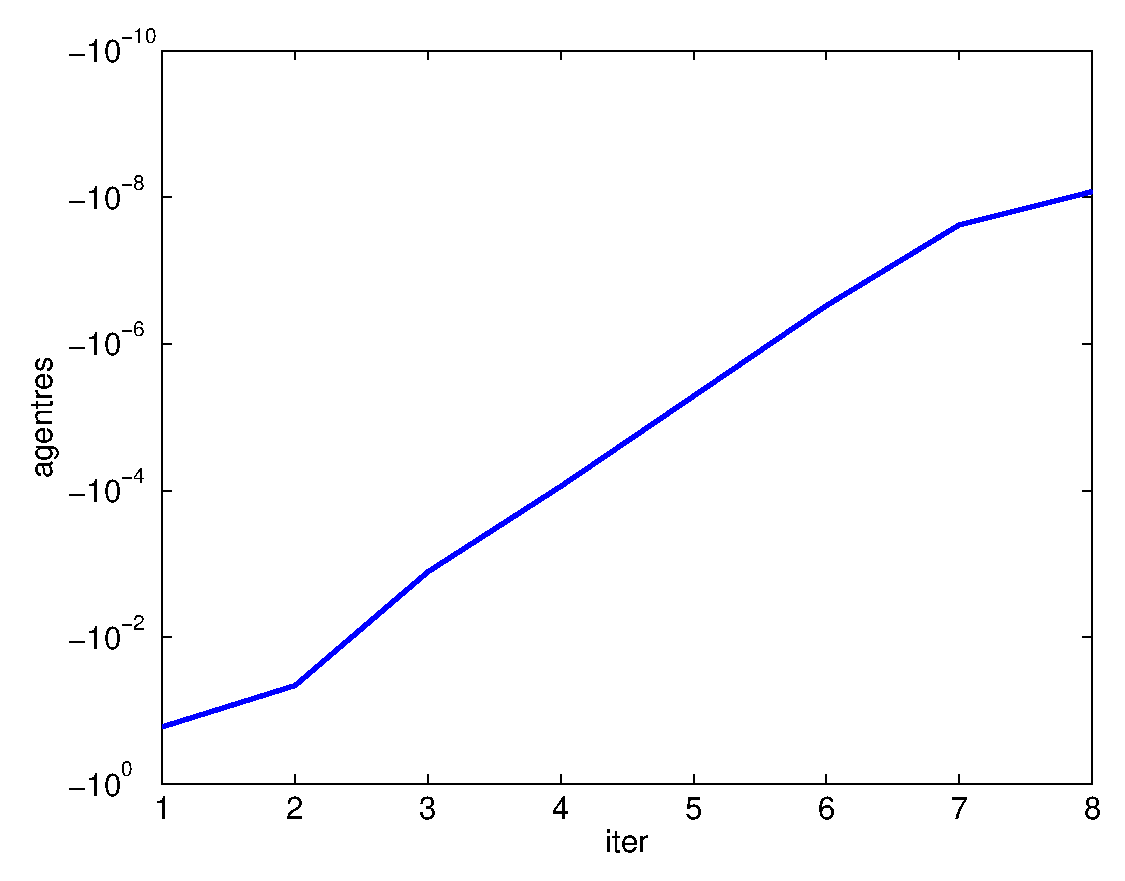
\includegraphics[width=0.6\linewidth]{matlab/agent_res.eps}
\end{center}
\caption{Agent residual versus trust region method iteration.}
\label{f-agent_res}
\end{figure}

Figure \ref{f-sparsity} shows the sparsity pattern of the
final solution $x$. Interestingly, only $56$ out of
$900$ good assignments are nonzero.

\begin{figure}
\begin{center}
\psfrag{agents}[b][t]{Agents}
\psfrag{goods}[t][b]{Goods}
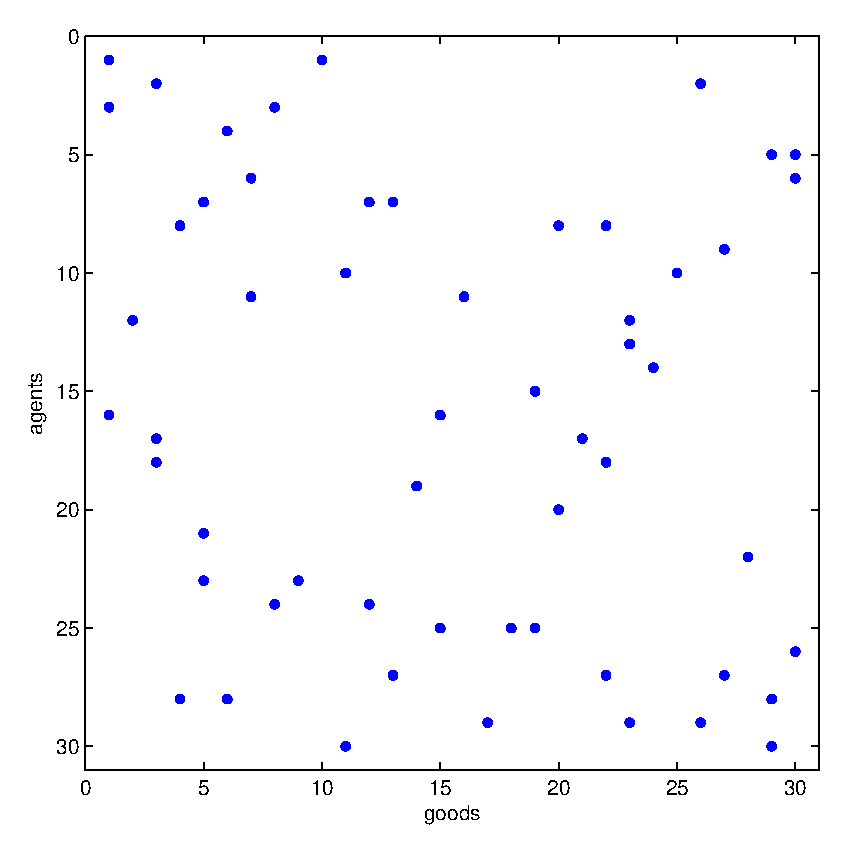
\includegraphics[width=0.6\linewidth]{matlab/sparsity.eps}
\end{center}
\caption{Sparsity pattern of final solution.}
\label{f-sparsity}
\end{figure}

XXX A word of caution: this method will oscillate if $\Delta_\mathrm{max}$
is too large. There are ways around this: we could expand $\exp(x)$
as a quadratic rather than just linearizing, or we could iteratively
decrease the trust region width.

\section{A Projected Subgradient Solution}

In this section we present a projected subgradient method for
solving problem (\ref{e-eq_prob_cvx}). We first reformulate
this problem as
\BEQ\label{e-eq_prob_cvx3}
\begin{array}{ll}
\mbox{minimize} & \max_{i,j} f_{ij}(x,\psi)\\
\mbox{subject to} & \sum_i x_{ij} = \sum_i b_{ij}, \quad \forall j\\
                  & x_{ij} \geq 0,
\end{array}
\EEQ
where
\[
f_{ij}(x,\psi) = \left(-\sum_k a_{ik} x_{ik} + a_{ij} \sum_{k} 
		  b_{ik} e^{\psi_k-\psi_j}\right).
\]
This is a convex optimization problem with a non-differentiable
objective function. However, all $f_{ij}$ are differentiable
and we have
\[
\frac{\partial f_{ij}(x,\psi)}{\partial x_{kl}} = \left\{
\begin{array}{ll}
-a_{il}, &\mbox{if $i=k$,}\\
0,       &\mbox{otherwise,}
\end{array}\right.
\]
and
\[
\frac{\partial f_{ij}(x,\psi)}{\partial \psi_k} = \left\{
\begin{array}{ll}
a_{ij}b_{ik}e^{\psi_k-\psi_j}, &\mbox{if $k\neq j$,}\\
-a_{ij}\sum_{l\neq k}b_{il}e^{\psi_l-\psi_j},       &\mbox{otherwise.}
\end{array}\right.
\]
 
\end{document}
